\documentclass{standalone}
\usepackage[T1]{fontenc}\usepackage{tikz}
\usepackage{amsmath, amsfonts}
\usetikzlibrary{arrows.meta}
\begin{document}
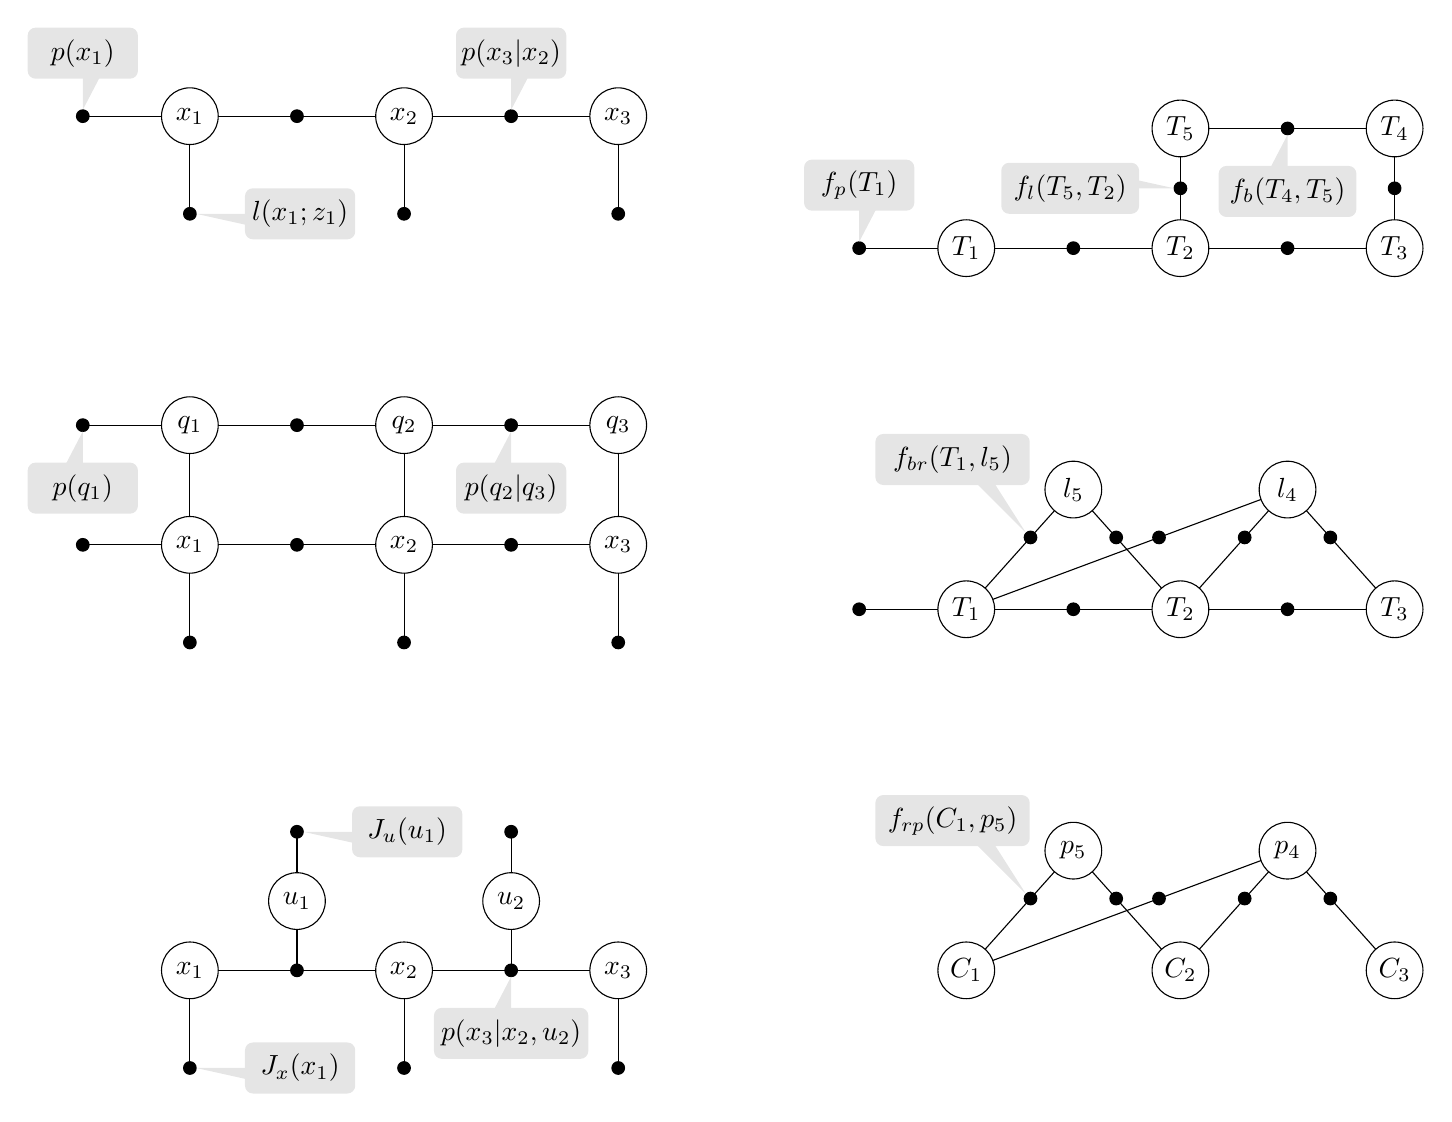
\begin{tikzpicture}
\draw[] (0.000000, 10.848000) circle (0.360000);
\node[] at (0.000000,10.848000) {$x_1$};
\draw[] (2.720000, 10.848000) circle (0.360000);
\node[] at (2.720000,10.848000) {$x_2$};
\draw[] (5.440000, 10.848000) circle (0.360000);
\node[] at (5.440000,10.848000) {$x_3$};
\draw[fill=black] (1.360000, 10.848000) circle (0.080000);
\draw[fill=black] (4.080000, 10.848000) circle (0.080000);
\draw[fill=black] (-1.360000, 10.848000) circle (0.080000);
\draw[fill=black] (0.000000, 9.608000) circle (0.080000);
\draw[fill=black] (2.720000, 9.608000) circle (0.080000);
\draw[fill=black] (5.440000, 9.608000) circle (0.080000);
\draw[] (0.360000, 10.848000) -- (2.360000, 10.848000);
\draw[] (3.080000, 10.848000) -- (5.080000, 10.848000);
\draw[] (-1.280000, 10.848000) -- (-0.360000, 10.848000);
\draw[] (0.000000, 9.688000) -- (-0.000000, 10.488000);
\draw[] (2.720000, 9.688000) -- (2.720000, 10.488000);
\draw[] (5.440000, 9.688000) -- (5.440000, 10.488000);
\draw[rounded corners=0.100000cm, fill=gray!20, draw=none] (-2.060000, 11.972000) -- (-0.660000, 11.972000) -- (-0.660000, 11.324000) -- (-2.060000, 11.324000) -- cycle;
\draw[fill=gray!20, draw=none] (-1.360000, 10.928000) -- (-1.360000, 11.648000) -- (-1.128596, 11.372224) -- cycle;
\node[] at (-1.360000,11.648000) {$p(x_1)$};
\draw[rounded corners=0.100000cm, fill=gray!20, draw=none] (0.700000, 9.932000) -- (2.100000, 9.932000) -- (2.100000, 9.284000) -- (0.700000, 9.284000) -- cycle;
\draw[fill=gray!20, draw=none] (0.080000, 9.608000) -- (1.400000, 9.608000) -- (1.124224, 9.376596) -- cycle;
\node[] at (1.400000,9.608000) {$l(x_1; z_1)$};
\draw[rounded corners=0.100000cm, fill=gray!20, draw=none] (3.380000, 11.972000) -- (4.780000, 11.972000) -- (4.780000, 11.324000) -- (3.380000, 11.324000) -- cycle;
\draw[fill=gray!20, draw=none] (4.080000, 10.928000) -- (4.080000, 11.648000) -- (4.311404, 11.372224) -- cycle;
\node[] at (4.080000,11.648000) {$p(x_3 | x_2)$};
\draw[] (0.000000, 5.404000) circle (0.360000);
\node[] at (0.000000,5.404000) {$x_1$};
\draw[] (2.720000, 5.404000) circle (0.360000);
\node[] at (2.720000,5.404000) {$x_2$};
\draw[] (5.440000, 5.404000) circle (0.360000);
\node[] at (5.440000,5.404000) {$x_3$};
\draw[] (0.000000, 6.924000) circle (0.360000);
\node[] at (0.000000,6.924000) {$q_1$};
\draw[] (2.720000, 6.924000) circle (0.360000);
\node[] at (2.720000,6.924000) {$q_2$};
\draw[] (5.440000, 6.924000) circle (0.360000);
\node[] at (5.440000,6.924000) {$q_3$};
\draw[fill=black] (1.360000, 5.404000) circle (0.080000);
\draw[fill=black] (4.080000, 5.404000) circle (0.080000);
\draw[fill=black] (-1.360000, 5.404000) circle (0.080000);
\draw[fill=black] (0.000000, 4.164000) circle (0.080000);
\draw[fill=black] (2.720000, 4.164000) circle (0.080000);
\draw[fill=black] (5.440000, 4.164000) circle (0.080000);
\draw[fill=black] (1.360000, 6.924000) circle (0.080000);
\draw[fill=black] (4.080000, 6.924000) circle (0.080000);
\draw[fill=black] (-1.360000, 6.924000) circle (0.080000);
\draw[] (0.360000, 5.404000) -- (2.360000, 5.404000);
\draw[] (3.080000, 5.404000) -- (5.080000, 5.404000);
\draw[] (-1.280000, 5.404000) -- (-0.360000, 5.404000);
\draw[] (0.000000, 4.244000) -- (-0.000000, 5.044000);
\draw[] (2.720000, 4.244000) -- (2.720000, 5.044000);
\draw[] (5.440000, 4.244000) -- (5.440000, 5.044000);
\draw[] (0.360000, 6.924000) -- (2.360000, 6.924000);
\draw[] (3.080000, 6.924000) -- (5.080000, 6.924000);
\draw[] (-1.280000, 6.924000) -- (-0.360000, 6.924000);
\draw[] (0.000000, 5.764000) -- (-0.000000, 6.564000);
\draw[] (2.720000, 5.764000) -- (2.720000, 6.564000);
\draw[] (5.440000, 5.764000) -- (5.440000, 6.564000);
\draw[rounded corners=0.100000cm, fill=gray!20, draw=none] (-2.060000, 6.448000) -- (-0.660000, 6.448000) -- (-0.660000, 5.800000) -- (-2.060000, 5.800000) -- cycle;
\draw[fill=gray!20, draw=none] (-1.360000, 6.844000) -- (-1.360000, 6.124000) -- (-1.591404, 6.399776) -- cycle;
\node[] at (-1.360000,6.124000) {$p(q_1)$};
\draw[rounded corners=0.100000cm, fill=gray!20, draw=none] (3.380000, 6.448000) -- (4.780000, 6.448000) -- (4.780000, 5.800000) -- (3.380000, 5.800000) -- cycle;
\draw[fill=gray!20, draw=none] (4.080000, 6.844000) -- (4.080000, 6.124000) -- (3.848596, 6.399776) -- cycle;
\node[] at (4.080000,6.124000) {$p(q_2| q_3)$};
\draw[] (0.000000, 0.000000) circle (0.360000);
\node[] at (0.000000,0.000000) {$x_1$};
\draw[] (2.720000, 0.000000) circle (0.360000);
\node[] at (2.720000,0.000000) {$x_2$};
\draw[] (5.440000, 0.000000) circle (0.360000);
\node[] at (5.440000,0.000000) {$x_3$};
\draw[] (1.360000, 0.880000) circle (0.360000);
\node[] at (1.360000,0.880000) {$u_1$};
\draw[] (4.080000, 0.880000) circle (0.360000);
\node[] at (4.080000,0.880000) {$u_2$};
\draw[fill=black] (1.360000, 0.000000) circle (0.080000);
\draw[fill=black] (4.080000, 0.000000) circle (0.080000);
\draw[fill=black] (0.000000, -1.240000) circle (0.080000);
\draw[fill=black] (2.720000, -1.240000) circle (0.080000);
\draw[fill=black] (5.440000, -1.240000) circle (0.080000);
\draw[fill=black] (1.360000, 1.760000) circle (0.080000);
\draw[fill=black] (4.080000, 1.760000) circle (0.080000);
\draw[] (0.360000, 0.000000) -- (2.360000, 0.000000);
\draw[] (3.080000, 0.000000) -- (5.080000, 0.000000);
\draw[] (0.000000, -1.160000) -- (-0.000000, -0.360000);
\draw[] (2.720000, -1.160000) -- (2.720000, -0.360000);
\draw[] (5.440000, -1.160000) -- (5.440000, -0.360000);
\draw[] (1.360000, 0.080000) -- (1.360000, 0.520000);
\draw[] (1.360000, 1.680000) -- (1.360000, 1.240000);
\draw[] (4.080000, 0.080000) -- (4.080000, 0.520000);
\draw[] (4.080000, 1.680000) -- (4.080000, 1.240000);
\draw[rounded corners=0.100000cm, fill=gray!20, draw=none] (0.700000, -0.916000) -- (2.100000, -0.916000) -- (2.100000, -1.564000) -- (0.700000, -1.564000) -- cycle;
\draw[fill=gray!20, draw=none] (0.080000, -1.240000) -- (1.400000, -1.240000) -- (1.124224, -1.471404) -- cycle;
\node[] at (1.400000,-1.240000) {$J_x(x_1)$};
\draw[rounded corners=0.100000cm, fill=gray!20, draw=none] (2.060000, 2.084000) -- (3.460000, 2.084000) -- (3.460000, 1.436000) -- (2.060000, 1.436000) -- cycle;
\draw[fill=gray!20, draw=none] (1.440000, 1.760000) -- (2.760000, 1.760000) -- (2.484224, 1.528596) -- cycle;
\node[] at (2.760000,1.760000) {$J_u(u_1)$};
\draw[rounded corners=0.100000cm, fill=gray!20, draw=none] (3.100000, -0.476000) -- (5.060000, -0.476000) -- (5.060000, -1.124000) -- (3.100000, -1.124000) -- cycle;
\draw[fill=gray!20, draw=none] (4.080000, -0.080000) -- (4.080000, -0.800000) -- (3.848596, -0.524224) -- cycle;
\node[] at (4.080000,-0.800000) {$p(x_3| x_2, u_2)$};
\draw[] (9.860000, 9.171899) circle (0.360000);
\node[] at (9.860000,9.171899) {$T_1$};
\draw[] (12.580000, 9.171899) circle (0.360000);
\node[] at (12.580000,9.171899) {$T_2$};
\draw[] (15.300000, 9.171899) circle (0.360000);
\node[] at (15.300000,9.171899) {$T_3$};
\draw[] (15.300000, 10.691899) circle (0.360000);
\node[] at (15.300000,10.691899) {$T_4$};
\draw[] (12.580000, 10.691899) circle (0.360000);
\node[] at (12.580000,10.691899) {$T_5$};
\draw[fill=black] (11.220000, 9.171899) circle (0.080000);
\draw[fill=black] (13.940000, 9.171899) circle (0.080000);
\draw[fill=black] (8.500000, 9.171899) circle (0.080000);
\draw[fill=black] (12.580000, 9.931899) circle (0.080000);
\draw[fill=black] (15.300000, 9.931899) circle (0.080000);
\draw[fill=black] (13.940000, 10.691899) circle (0.080000);
\draw[] (10.220000, 9.171899) -- (12.220000, 9.171899);
\draw[] (12.940000, 9.171899) -- (14.940000, 9.171899);
\draw[] (8.580000, 9.171899) -- (9.500000, 9.171899);
\draw[] (12.580000, 9.531899) -- (12.580000, 10.331899);
\draw[] (15.300000, 9.531899) -- (15.300000, 10.331899);
\draw[] (14.940000, 10.691899) -- (12.940000, 10.691899);
\draw[rounded corners=0.100000cm, fill=gray!20, draw=none] (7.800000, 10.295899) -- (9.200000, 10.295899) -- (9.200000, 9.647899) -- (7.800000, 9.647899) -- cycle;
\draw[fill=gray!20, draw=none] (8.500000, 9.251899) -- (8.500000, 9.971899) -- (8.731404, 9.696123) -- cycle;
\node[] at (8.500000,9.971899) {$f_p(T_1)$};
\draw[rounded corners=0.100000cm, fill=gray!20, draw=none] (10.305000, 10.255899) -- (12.055000, 10.255899) -- (12.055000, 9.607899) -- (10.305000, 9.607899) -- cycle;
\draw[fill=gray!20, draw=none] (12.500000, 9.931899) -- (11.180000, 9.931899) -- (11.455776, 10.163303) -- cycle;
\node[] at (11.180000,9.931899) {$f_l(T_5, T_2)$};
\draw[rounded corners=0.100000cm, fill=gray!20, draw=none] (13.065000, 10.215899) -- (14.815000, 10.215899) -- (14.815000, 9.567899) -- (13.065000, 9.567899) -- cycle;
\draw[fill=gray!20, draw=none] (13.940000, 10.611899) -- (13.940000, 9.891899) -- (13.708596, 10.167675) -- cycle;
\node[] at (13.940000,9.891899) {$f_b(T_4, T_5)$};
\draw[] (9.860000, 4.585949) circle (0.360000);
\node[] at (9.860000,4.585949) {$T_1$};
\draw[] (12.580000, 4.585949) circle (0.360000);
\node[] at (12.580000,4.585949) {$T_2$};
\draw[] (15.300000, 4.585949) circle (0.360000);
\node[] at (15.300000,4.585949) {$T_3$};
\draw[] (13.940000, 6.105949) circle (0.360000);
\node[] at (13.940000,6.105949) {$l_4$};
\draw[] (11.220000, 6.105949) circle (0.360000);
\node[] at (11.220000,6.105949) {$l_5$};
\draw[fill=black] (11.220000, 4.585949) circle (0.080000);
\draw[fill=black] (13.940000, 4.585949) circle (0.080000);
\draw[fill=black] (8.500000, 4.585949) circle (0.080000);
\draw[fill=black] (10.676000, 5.497949) circle (0.080000);
\draw[fill=black] (11.764000, 5.497949) circle (0.080000);
\draw[fill=black] (13.396000, 5.497949) circle (0.080000);
\draw[fill=black] (14.484000, 5.497949) circle (0.080000);
\draw[fill=black] (12.308000, 5.497949) circle (0.080000);
\draw[] (10.220000, 4.585949) -- (12.220000, 4.585949);
\draw[] (12.940000, 4.585949) -- (14.940000, 4.585949);
\draw[] (8.580000, 4.585949) -- (9.500000, 4.585949);
\draw[] (10.100046, 4.854236) -- (10.979954, 5.837663);
\draw[] (12.339954, 4.854236) -- (11.460046, 5.837663);
\draw[] (12.820046, 4.854236) -- (13.699954, 5.837663);
\draw[] (15.059954, 4.854236) -- (14.180046, 5.837663);
\draw[] (10.197350, 4.711629) -- (13.602650, 5.980270);
\draw[rounded corners=0.100000cm, fill=gray!20, draw=none] (8.706051, 6.811899) -- (10.666051, 6.811899) -- (10.666051, 6.163899) -- (8.706051, 6.163899) -- cycle;
\draw[fill=gray!20, draw=none] (10.619431, 5.554518) -- (9.686051, 6.487899) -- (10.044681, 6.456523) -- cycle;
\node[] at (9.686051,6.487899) {$f_{br}(T_1, l_5)$};
\draw[] (9.860000, 0.000000) circle (0.360000);
\node[] at (9.860000,0.000000) {$C_1$};
\draw[] (12.580000, 0.000000) circle (0.360000);
\node[] at (12.580000,0.000000) {$C_2$};
\draw[] (15.300000, 0.000000) circle (0.360000);
\node[] at (15.300000,0.000000) {$C_3$};
\draw[] (13.940000, 1.520000) circle (0.360000);
\node[] at (13.940000,1.520000) {$p_4$};
\draw[] (11.220000, 1.520000) circle (0.360000);
\node[] at (11.220000,1.520000) {$p_5$};
\draw[fill=black] (10.676000, 0.912000) circle (0.080000);
\draw[fill=black] (11.764000, 0.912000) circle (0.080000);
\draw[fill=black] (13.396000, 0.912000) circle (0.080000);
\draw[fill=black] (14.484000, 0.912000) circle (0.080000);
\draw[fill=black] (12.308000, 0.912000) circle (0.080000);
\draw[] (10.100046, 0.268287) -- (10.979954, 1.251713);
\draw[] (12.339954, 0.268287) -- (11.460046, 1.251713);
\draw[] (12.820046, 0.268287) -- (13.699954, 1.251713);
\draw[] (15.059954, 0.268287) -- (14.180046, 1.251713);
\draw[] (10.197350, 0.125679) -- (13.602650, 1.394321);
\draw[rounded corners=0.100000cm, fill=gray!20, draw=none] (8.706051, 2.225949) -- (10.666051, 2.225949) -- (10.666051, 1.577949) -- (8.706051, 1.577949) -- cycle;
\draw[fill=gray!20, draw=none] (10.619431, 0.968569) -- (9.686051, 1.901949) -- (10.044681, 1.870573) -- cycle;
\node[] at (9.686051,1.901949) {$f_{rp}(C_1, p_5)$};
\end{tikzpicture}
\end{document}
